% Topic 3.2: Blockchain Mechanics
% Digital Finance Introduction
\documentclass[11pt,aspectratio=169]{beamer}
\usetheme{Madrid}

% ======================= PACKAGES =======================
\usepackage{graphicx}
\usepackage{booktabs}
\usepackage{adjustbox}
\usepackage{multicol}
\usepackage{amsmath}
\usepackage{amssymb}
\usepackage{tikz}
\usetikzlibrary{arrows,shapes,positioning,shadows,trees}
\usepackage{listings}
\usepackage{xcolor}

% ======================= COLOR DEFINITIONS =======================
% Primary color scheme: Blue/Teal for Digital Finance
\definecolor{dfblue}{RGB}{0,102,204}
\definecolor{dfteal}{RGB}{0,153,153}
\definecolor{dfcyan}{RGB}{51,187,204}
\definecolor{dflightblue}{RGB}{153,204,255}
\definecolor{dflightblue2}{RGB}{173,214,255}
\definecolor{dflightblue3}{RGB}{193,224,255}
\definecolor{dflightblue4}{RGB}{213,234,255}

% Accent colors for finance applications
\definecolor{dfgreen}{RGB}{44, 160, 44}
\definecolor{dfred}{RGB}{214, 39, 40}
\definecolor{dforange}{RGB}{255, 127, 14}
\definecolor{dfgray}{RGB}{127, 127, 127}

% Utility colors
\definecolor{lightgray}{RGB}{240, 240, 240}
\definecolor{midgray}{RGB}{180, 180, 180}
\definecolor{codebg}{RGB}{245, 245, 245}

% ======================= THEME CUSTOMIZATION =======================
% Apply Digital Finance color scheme to Madrid theme
\setbeamercolor{palette primary}{bg=dflightblue3,fg=dfblue}
\setbeamercolor{palette secondary}{bg=dflightblue2,fg=dfblue}
\setbeamercolor{palette tertiary}{bg=dfteal,fg=white}
\setbeamercolor{palette quaternary}{bg=dfblue,fg=white}

\setbeamercolor{structure}{fg=dfblue}
\setbeamercolor{section in toc}{fg=dfblue}
\setbeamercolor{subsection in toc}{fg=dfteal}
\setbeamercolor{title}{fg=dfblue}
\setbeamercolor{frametitle}{fg=dfblue,bg=dflightblue3}
\setbeamercolor{block title}{bg=dflightblue2,fg=dfblue}
\setbeamercolor{block body}{bg=dflightblue4,fg=black}

% Remove navigation symbols for cleaner look
\setbeamertemplate{navigation symbols}{}

% Clean itemize/enumerate
\setbeamertemplate{itemize items}[circle]
\setbeamertemplate{enumerate items}[default]

% Margins for readability
\setbeamersize{text margin left=8mm,text margin right=8mm}

% ======================= LISTINGS CONFIGURATION =======================
% Python code style
\lstdefinestyle{pythonstyle}{
    language=Python,
    basicstyle=\ttfamily\footnotesize,
    keywordstyle=\color{dfblue}\bfseries,
    stringstyle=\color{dforange},
    commentstyle=\color{dfgray}\itshape,
    numberstyle=\tiny\color{dfgray},
    numbers=left,
    numbersep=5pt,
    backgroundcolor=\color{codebg},
    showspaces=false,
    showstringspaces=false,
    showtabs=false,
    frame=single,
    rulecolor=\color{midgray},
    tabsize=4,
    captionpos=b,
    breaklines=true,
    breakatwhitespace=false,
    escapeinside={(*@}{@*)},
    xleftmargin=10pt,
    xrightmargin=10pt
}

% Solidity code style
\lstdefinestyle{soliditystyle}{
    language=Java, % closest approximation
    basicstyle=\ttfamily\footnotesize,
    keywordstyle=\color{dfteal}\bfseries,
    stringstyle=\color{dforange},
    commentstyle=\color{dfgray}\itshape,
    numberstyle=\tiny\color{dfgray},
    numbers=left,
    numbersep=5pt,
    backgroundcolor=\color{codebg},
    showspaces=false,
    showstringspaces=false,
    showtabs=false,
    frame=single,
    rulecolor=\color{midgray},
    tabsize=2,
    captionpos=b,
    breaklines=true,
    breakatwhitespace=false,
    escapeinside={(*@}{@*)},
    xleftmargin=10pt,
    xrightmargin=10pt,
    morekeywords={pragma, contract, function, returns, public, private, view, pure, payable, address, uint256, mapping, event, modifier}
}

% Inline code command
\newcommand{\code}[1]{\texttt{\color{dfblue}#1}}

% ======================= CUSTOM COMMANDS =======================
% Bottom annotation (Madrid-style)
\newcommand{\bottomnote}[1]{%
\vfill
\vspace{-2mm}
\textcolor{dflightblue2}{\rule{\textwidth}{0.4pt}}
\vspace{1mm}
\footnotesize
\textbf{#1}
}

% Compact list spacing
\newcommand{\compactlist}{%
\setlength{\itemsep}{0pt}%
\setlength{\parskip}{0pt}%
\setlength{\parsep}{0pt}%
}

% Chart placeholder
\newcommand{\chartplaceholder}[2][5cm]{%
\begin{center}
\begin{adjustbox}{max width=0.95\textwidth, max height=#1}
\framebox[\textwidth][c]{%
\rule{0pt}{#1}%
\textcolor{midgray}{[#2]}%
}
\end{adjustbox}
\end{center}
}

% ======================= FINANCE NOTATION MACROS =======================
% Probability and statistics
\newcommand{\E}{\mathbb{E}} % Expected value
\newcommand{\Var}{\mathrm{Var}} % Variance
\newcommand{\Cov}{\mathrm{Cov}} % Covariance
\newcommand{\Prob}{\mathbb{P}} % Probability

% Distributions
\newcommand{\Normal}{\mathcal{N}} % Normal distribution
\newcommand{\Uniform}{\mathcal{U}} % Uniform distribution

% Returns and prices
\newcommand{\Ret}{R} % Return
\newcommand{\LogRet}{r} % Log return
\newcommand{\Price}{S} % Price/Stock price
\newcommand{\Strike}{K} % Strike price

% Options and derivatives
\newcommand{\CallPrice}{C} % Call option price
\newcommand{\PutPrice}{P} % Put option price
\newcommand{\Greeks}[1]{\mathit{#1}} % Greek letters

% Risk measures
\newcommand{\VaR}{\mathrm{VaR}} % Value at Risk
\newcommand{\CVaR}{\mathrm{CVaR}} % Conditional VaR
\newcommand{\Sharpe}{\mathrm{SR}} % Sharpe Ratio

% Time series
\newcommand{\AR}{\mathrm{AR}} % Autoregressive
\newcommand{\MA}{\mathrm{MA}} % Moving average
\newcommand{\GARCH}{\mathrm{GARCH}} % GARCH

% Blockchain/Crypto
\newcommand{\Hash}{\mathrm{Hash}} % Hash function
\newcommand{\Block}{\mathcal{B}} % Block
\newcommand{\Chain}{\mathcal{C}} % Chain

% Real numbers, integers
\newcommand{\R}{\mathbb{R}}
\newcommand{\Z}{\mathbb{Z}}
\newcommand{\N}{\mathbb{N}}

% ======================= TIKZ STYLES =======================
% Styles for finance-related diagrams
\tikzstyle{process} = [rectangle, minimum width=3cm, minimum height=1cm, text centered, draw=dfblue, fill=dflightblue4, thick]
\tikzstyle{decision} = [diamond, minimum width=3cm, minimum height=1cm, text centered, draw=dfteal, fill=dflightblue4, thick]
\tikzstyle{arrow} = [thick,->,>=stealth,color=dfblue]
\tikzstyle{blockchain} = [rectangle, rounded corners, minimum width=2.5cm, minimum height=1cm, text centered, draw=dfteal, fill=dflightblue3, thick]
\tikzstyle{transaction} = [circle, minimum size=0.8cm, text centered, draw=dforange, fill=dflightblue4, thick]

% ======================= FOOTER TEMPLATE =======================
\setbeamertemplate{footline}{
    \hbox{\begin{beamercolorbox}[wd=\paperwidth,ht=2.5ex,dp=1ex,leftskip=.5em,rightskip=.5em]{author in head/foot}
    \tiny
    \textbf{Digital Finance} \hfill
    Joerg Osterrieder \hfill
    \insertdate \hfill
    Page \insertframenumber{} / \inserttotalframenumber
    \end{beamercolorbox}}
}

% ======================= SECTION DIVIDER TEMPLATE =======================
\AtBeginSection[]{
\begin{frame}[plain]
\vfill
\centering
\begin{beamercolorbox}[sep=12pt,center]{title}
\usebeamerfont{title}\LARGE\insertsection\par
\end{beamercolorbox}
\vfill
\end{frame}
}


% Additional TikZ libraries for blockchain diagrams
\usetikzlibrary{chains,calc,decorations.pathreplacing,fit,backgrounds}

% Custom styles for blockchain diagrams
\tikzstyle{blocknode} = [rectangle, rounded corners, minimum width=3cm, minimum height=2cm, text centered, draw=dfteal, fill=dflightblue3, thick]
\tikzstyle{hashbox} = [rectangle, rounded corners, minimum width=2cm, minimum height=0.8cm, text centered, draw=dfteal, fill=dflightblue3, thick, font=\footnotesize]
\tikzstyle{databox} = [rectangle, minimum width=2.5cm, minimum height=0.6cm, text centered, draw=dfblue, fill=dflightblue4, thick, font=\footnotesize]
\tikzstyle{keybox} = [rectangle, rounded corners, minimum width=2cm, minimum height=0.6cm, text centered, draw=dforange, fill=dflightblue4, thick, font=\footnotesize]
\tikzstyle{walletbox} = [rectangle, rounded corners, minimum width=2.5cm, minimum height=1cm, text centered, draw=dfgreen, fill=dflightblue4, thick]
\tikzstyle{networknode} = [circle, draw=dfblue, fill=dflightblue4, minimum size=0.8cm, thick]

% ======================= DOCUMENT INFO =======================
\title[Topic 3.2: Blockchain Mechanics]{Topic 3.2: Blockchain Mechanics}
\subtitle{Consensus, Blocks, and the Trilemma}
\author{Joerg Osterrieder}
\institute{Digital Finance}
\date{2025}

\begin{document}

% =======================================================================
% SLIDE 1: TITLE SLIDE
% =======================================================================
\begin{frame}[plain]
\titlepage
\end{frame}

% =======================================================================
% SLIDE 2: LEARNING OBJECTIVES
% =======================================================================
\begin{frame}{Learning Objectives}
\textbf{By the end of this topic, you will be able to:}

\begin{enumerate}
\item \textbf{Define} what a blockchain is and explain its key properties (distributed, append-only, consensus-based)
\vspace{2mm}
\item \textbf{Describe} the structure of a block and how blocks are linked through cryptographic hashes
\vspace{2mm}
\item \textbf{Compare} Proof of Work (PoW) and Proof of Stake (PoS) consensus mechanisms
\vspace{2mm}
\item \textbf{Explain} the blockchain trilemma and why it creates fundamental design tradeoffs
\vspace{2mm}
\item \textbf{Evaluate} Layer 1 and Layer 2 scaling solutions
\end{enumerate}

\vspace{3mm}
\begin{block}{Core Question}
How do thousands of strangers agree on a single version of the truth without any central authority?
\end{block}
\end{frame}

% =======================================================================
% SLIDE 3: PREREQUISITES - CRYPTOGRAPHY RECAP 1
% =======================================================================
\begin{frame}{Prerequisites: Cryptography Concepts You'll Need}
\textbf{From Topic 3.1 -- Quick Recap:}

\begin{columns}[T]
\begin{column}{0.48\textwidth}
\textbf{Hash Functions}
\begin{itemize}\compactlist
\item Input $\rightarrow$ Fixed-size output (256 bits)
\item \textbf{Deterministic:} Same input = same output
\item \textbf{One-way:} Cannot reverse to find input
\item \textbf{Avalanche effect:} Tiny change = completely different output
\end{itemize}

\vspace{3mm}
\textit{Example:}\\
\texttt{"Hello"} $\rightarrow$ \texttt{185f8db3...}\\
\texttt{"Hello!"} $\rightarrow$ \texttt{334d016f...}
\end{column}
\begin{column}{0.48\textwidth}
\textbf{Digital Signatures}
\begin{itemize}\compactlist
\item Private key signs transactions
\item Public key verifies signatures
\item \textbf{Authentication:} Proves identity
\item \textbf{Non-repudiation:} Cannot deny signing
\end{itemize}

\vspace{3mm}
\textit{Key insight:}\\
Only the person with the private key can create a valid signature.
\end{column}
\end{columns}

\vspace{3mm}
\bottomnote{If these concepts are unfamiliar, review Topic 3.1 before continuing}
\end{frame}

% =======================================================================
% SLIDE 4: PREREQUISITES - WHY THIS MATTERS
% =======================================================================
\begin{frame}{Prerequisites: From Primitives to Systems}
\textbf{How cryptographic primitives enable blockchain:}

\begin{center}
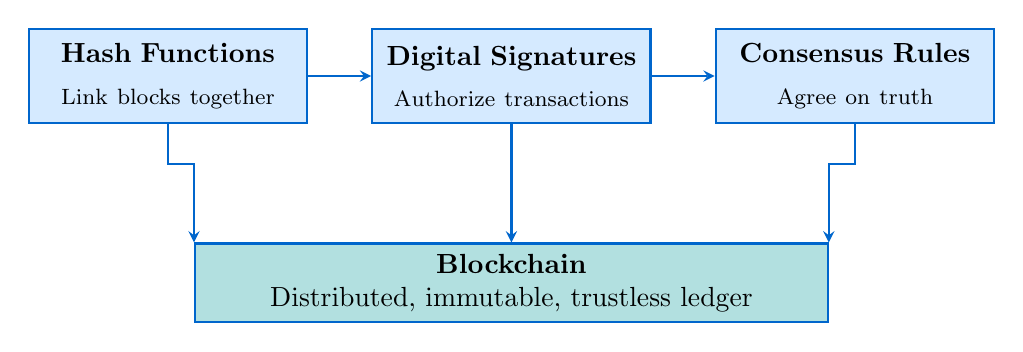
\begin{tikzpicture}[node distance=0.5cm]
% Three boxes
\node[process, minimum width=3.5cm, minimum height=1.2cm, text width=3.3cm, align=center] (hash) {
\textbf{Hash Functions}\\[1mm]
\footnotesize Link blocks together
};
\node[process, minimum width=3.5cm, minimum height=1.2cm, text width=3.3cm, align=center, right=0.8cm of hash] (sigs) {
\textbf{Digital Signatures}\\[1mm]
\footnotesize Authorize transactions
};
\node[process, minimum width=3.5cm, minimum height=1.2cm, text width=3.3cm, align=center, right=0.8cm of sigs] (consensus) {
\textbf{Consensus Rules}\\[1mm]
\footnotesize Agree on truth
};

\draw[arrow] (hash) -- (sigs);
\draw[arrow] (sigs) -- (consensus);

% Result
\node[process, below=1.5cm of sigs, minimum width=8cm, fill=dfteal!30, text width=7.8cm, align=center] (result) {
\textbf{Blockchain}\\
Distributed, immutable, trustless ledger
};

\draw[arrow] (hash.south) -- ++(0,-0.5) -| (result.north west);
\draw[arrow] (sigs.south) -- (result.north);
\draw[arrow] (consensus.south) -- ++(0,-0.5) -| (result.north east);
\end{tikzpicture}
\end{center}

\vspace{3mm}
\textbf{Today's focus:} How these pieces fit together to create a system that works without trusted intermediaries.
\end{frame}

% =======================================================================
% SLIDE 5: WHAT IS A BLOCKCHAIN?
% =======================================================================
\begin{frame}{What Is a Blockchain?}
\begin{center}
\textit{``A blockchain is a distributed ledger that is append-only,\\cryptographically linked, and maintained by consensus.''}
\end{center}

\vspace{5mm}
\begin{columns}[T]
\begin{column}{0.32\textwidth}
\textbf{Distributed}
\begin{itemize}\compactlist
\item No central server
\item Thousands of copies
\item No single point of failure
\end{itemize}
\end{column}
\begin{column}{0.32\textwidth}
\textbf{Append-Only}
\begin{itemize}\compactlist
\item Can only add data
\item Cannot modify history
\item Immutable record
\end{itemize}
\end{column}
\begin{column}{0.32\textwidth}
\textbf{Consensus-Based}
\begin{itemize}\compactlist
\item Network agrees on state
\item No trusted authority
\item Rules enforced by code
\end{itemize}
\end{column}
\end{columns}

\vspace{5mm}
\begin{center}
\fbox{\parbox{0.75\textwidth}{\centering
\textbf{Simple analogy:} A shared Google Doc that everyone can read,\\
only append to, and no one can delete from
}}
\end{center}
\end{frame}

% =======================================================================
% SLIDE 6: BLOCKCHAIN STRUCTURE - VISUAL
% =======================================================================
\begin{frame}{Blockchain Structure: Blocks Linked by Hashes}
\begin{center}
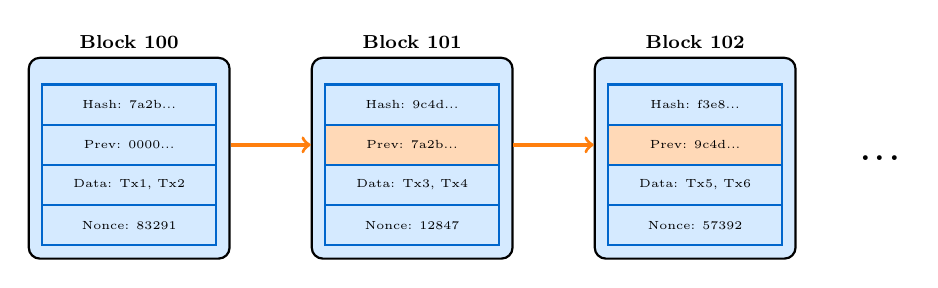
\begin{tikzpicture}[node distance=0.3cm, scale=0.85, transform shape]
% Block 1
\node[draw, thick, rounded corners, minimum width=3cm, minimum height=3cm, fill=dflightblue4] (b1) {};
\node[above=0mm of b1.north, font=\bfseries\footnotesize] {Block 100};
\node[databox, minimum width=2.6cm, font=\tiny] at ($(b1.center) + (0,0.8)$) {Hash: 7a2b...};
\node[databox, minimum width=2.6cm, font=\tiny] at ($(b1.center) + (0,0.2)$) {Prev: 0000...};
\node[databox, minimum width=2.6cm, font=\tiny] at ($(b1.center) + (0,-0.4)$) {Data: Tx1, Tx2};
\node[databox, minimum width=2.6cm, font=\tiny] at ($(b1.center) + (0,-1)$) {Nonce: 83291};

% Block 2
\node[draw, thick, rounded corners, minimum width=3cm, minimum height=3cm, fill=dflightblue4, right=1.2cm of b1] (b2) {};
\node[above=0mm of b2.north, font=\bfseries\footnotesize] {Block 101};
\node[databox, minimum width=2.6cm, font=\tiny] at ($(b2.center) + (0,0.8)$) {Hash: 9c4d...};
\node[databox, minimum width=2.6cm, font=\tiny, fill=dforange!30] at ($(b2.center) + (0,0.2)$) {Prev: 7a2b...};
\node[databox, minimum width=2.6cm, font=\tiny] at ($(b2.center) + (0,-0.4)$) {Data: Tx3, Tx4};
\node[databox, minimum width=2.6cm, font=\tiny] at ($(b2.center) + (0,-1)$) {Nonce: 12847};

% Block 3
\node[draw, thick, rounded corners, minimum width=3cm, minimum height=3cm, fill=dflightblue4, right=1.2cm of b2] (b3) {};
\node[above=0mm of b3.north, font=\bfseries\footnotesize] {Block 102};
\node[databox, minimum width=2.6cm, font=\tiny] at ($(b3.center) + (0,0.8)$) {Hash: f3e8...};
\node[databox, minimum width=2.6cm, font=\tiny, fill=dforange!30] at ($(b3.center) + (0,0.2)$) {Prev: 9c4d...};
\node[databox, minimum width=2.6cm, font=\tiny] at ($(b3.center) + (0,-0.4)$) {Data: Tx5, Tx6};
\node[databox, minimum width=2.6cm, font=\tiny] at ($(b3.center) + (0,-1)$) {Nonce: 57392};

% Linking arrows
\draw[very thick, dforange, ->] ($(b1.east) + (0,0.2)$) -- ($(b2.west) + (0,0.2)$);
\draw[very thick, dforange, ->] ($(b2.east) + (0,0.2)$) -- ($(b3.west) + (0,0.2)$);

% Future blocks
\node[right=0.8cm of b3, font=\Huge] {...};
\end{tikzpicture}
\end{center}

\vspace{3mm}
\textbf{The chain property:} Each block contains the hash of the previous block

\textbf{Why this matters:} Change Block 100 $\rightarrow$ its hash changes $\rightarrow$ Block 101's ``Prev'' becomes invalid $\rightarrow$ cascading invalidity

\bottomnote{This is why blockchain history is considered immutable}
\end{frame}

% =======================================================================
% SLIDE 7: BLOCK COMPONENTS
% =======================================================================
\begin{frame}{Anatomy of a Block}
\begin{columns}[T]
\begin{column}{0.55\textwidth}
\textbf{Every block contains:}

\begin{description}
\item[Index] Position in the chain (Block 0, 1, 2...)
\item[Timestamp] When the block was created
\item[Data] Transactions or other content
\item[Previous Hash] Link to the prior block
\item[Nonce] Number used for mining
\item[Hash] The block's unique fingerprint
\end{description}

\vspace{3mm}
\textbf{Key insight:} The hash is calculated from ALL other fields. Change any field, and the hash changes completely.
\end{column}
\begin{column}{0.42\textwidth}
\begin{center}
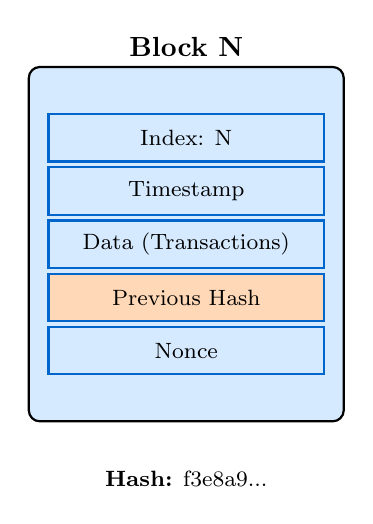
\begin{tikzpicture}[scale=0.9]
\node[draw, thick, rounded corners, minimum width=4cm, minimum height=4.5cm, fill=dflightblue4] (block) {};
\node[above=0mm of block.north, font=\bfseries] {Block N};

\node[databox, minimum width=3.5cm] at ($(block.center) + (0,1.5)$) {Index: N};
\node[databox, minimum width=3.5cm] at ($(block.center) + (0,0.75)$) {Timestamp};
\node[databox, minimum width=3.5cm] at ($(block.center) + (0,0)$) {Data (Transactions)};
\node[databox, minimum width=3.5cm, fill=dforange!30] at ($(block.center) + (0,-0.75)$) {Previous Hash};
\node[databox, minimum width=3.5cm] at ($(block.center) + (0,-1.5)$) {Nonce};

\node[below=5mm of block.south, font=\footnotesize] {\textbf{Hash:} f3e8a9...};
\end{tikzpicture}
\end{center}
\end{column}
\end{columns}
\end{frame}

% =======================================================================
% SLIDE 8: THE GENESIS BLOCK
% =======================================================================
\begin{frame}{The Genesis Block: Where It All Begins}
\begin{columns}[T]
\begin{column}{0.55\textwidth}
\textbf{What is the Genesis Block?}
\begin{itemize}
\item The \textbf{first block} in any blockchain
\item Has no previous block to reference
\item ``Previous Hash'' is typically all zeros
\item Created when the blockchain launches
\end{itemize}

\vspace{3mm}
\textbf{Bitcoin's Genesis Block}
\begin{itemize}
\item Mined January 3, 2009
\item Block 0 -- the very first
\item Contains a hidden message from Satoshi Nakamoto
\end{itemize}
\end{column}
\begin{column}{0.42\textwidth}
\begin{center}
\fbox{\parbox{0.95\textwidth}{
\textbf{Bitcoin Genesis Block Message:}\\[2mm]
\footnotesize\textit{``The Times 03/Jan/2009 Chancellor on brink of second bailout for banks''}\\[2mm]
\normalsize This headline proved the block wasn't created earlier and made a political statement about the financial system.
}}
\end{center}
\end{column}
\end{columns}

\vspace{3mm}
\bottomnote{Every blockchain traces back to its genesis block -- the root of the chain}
\end{frame}

% =======================================================================
% SLIDE 9: WHY TAMPERING IS DETECTABLE
% =======================================================================
\begin{frame}{Why Tampering Is Detectable}
\begin{center}
\begin{tabular}{c|c}
\textbf{Original Chain} & \textbf{Tampered Chain} \\
\hline
& \\
Block 100: Hash = 7a2b... & Block 100: Hash = \textcolor{dfred}{x9f2...} \\
$\downarrow$ (valid link) & $\downarrow$ \textcolor{dfred}{(broken link!)} \\
Block 101: Prev = 7a2b... & Block 101: Prev = 7a2b... \textcolor{dfred}{X} \\
$\downarrow$ (valid link) & $\downarrow$ \textcolor{dfred}{(broken link!)} \\
Block 102: Prev = 9c4d... & Block 102: Prev = 9c4d... \textcolor{dfred}{X} \\
& \\
\textcolor{dfgreen}{\checkmark Valid} & \textcolor{dfred}{X Invalid} \\
\end{tabular}
\end{center}

\vspace{5mm}
\textbf{To tamper with history, an attacker must:}
\begin{enumerate}
\item Change the target block's data
\item Recalculate that block's hash
\item Recalculate \textit{every subsequent block's hash}
\item Do this faster than the honest network adds new blocks
\end{enumerate}

\textcolor{dfred}{Practically impossible once blocks are deep in the chain}
\end{frame}

% =======================================================================
% SLIDE 10: THE CONSENSUS PROBLEM
% =======================================================================
\begin{frame}{The Consensus Problem}
\begin{columns}[T]
\begin{column}{0.55\textwidth}
\textbf{The Challenge}

In a decentralized network:
\begin{itemize}
\item No central authority
\item Nodes don't trust each other
\item Messages can be delayed or lost
\item Some nodes may be malicious
\end{itemize}

\vspace{3mm}
\textbf{The Question}

How do thousands of strangers agree on:
\begin{itemize}
\item Which transactions are valid?
\item What order do they go in?
\item What is the ``true'' history?
\end{itemize}
\end{column}
\begin{column}{0.42\textwidth}
\begin{center}
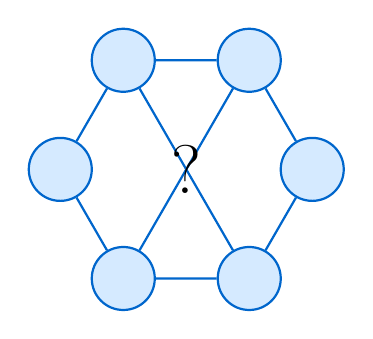
\begin{tikzpicture}[scale=0.8]
% Network of nodes
\foreach \i in {1,...,6} {
    \node[networknode] (n\i) at ({60*\i}:2) {};
}
% Some connections
\draw[thick, dfblue] (n1) -- (n2);
\draw[thick, dfblue] (n2) -- (n3);
\draw[thick, dfblue] (n3) -- (n4);
\draw[thick, dfblue] (n4) -- (n5);
\draw[thick, dfblue] (n5) -- (n6);
\draw[thick, dfblue] (n6) -- (n1);
\draw[thick, dfblue] (n1) -- (n4);
\draw[thick, dfblue] (n2) -- (n5);

% Question mark in center
\node[font=\Huge] at (0,0) {?};
\end{tikzpicture}

\footnotesize Who decides the truth?
\end{center}
\end{column}
\end{columns}

\vspace{3mm}
\begin{block}{Consensus Mechanism}
A set of rules that allows a distributed network to agree on a single version of truth, even in the presence of faulty or malicious participants.
\end{block}
\end{frame}

% =======================================================================
% SLIDE 11: DEFINING CONSENSUS MECHANISM
% =======================================================================
\begin{frame}{What Is a Consensus Mechanism?}
\textbf{Definition:} A protocol that enables distributed nodes to agree on the state of a shared ledger without requiring trust.

\vspace{5mm}
\begin{columns}[T]
\begin{column}{0.48\textwidth}
\textbf{Requirements:}
\begin{itemize}\compactlist
\item \textbf{Agreement:} All honest nodes accept the same transactions
\item \textbf{Validity:} Only valid transactions are accepted
\item \textbf{Termination:} Decisions are eventually made
\item \textbf{Fault Tolerance:} Works despite some bad actors
\end{itemize}
\end{column}
\begin{column}{0.48\textwidth}
\textbf{Main Approaches:}
\begin{itemize}\compactlist
\item \textbf{Proof of Work (PoW):} Computational puzzle solving
\item \textbf{Proof of Stake (PoS):} Economic collateral
\item \textbf{Proof of Authority:} Trusted validators
\item \textbf{BFT variants:} Voting-based
\end{itemize}
\end{column}
\end{columns}

\vspace{5mm}
\begin{center}
\fbox{\parbox{0.8\textwidth}{\centering
\textbf{Key insight:} Different consensus mechanisms make different tradeoffs between security, speed, decentralization, and energy use.
}}
\end{center}
\end{frame}

% =======================================================================
% SLIDE 12: PROOF OF WORK - VISUAL
% =======================================================================
\begin{frame}{Proof of Work (PoW): Bitcoin's Answer}
\begin{center}
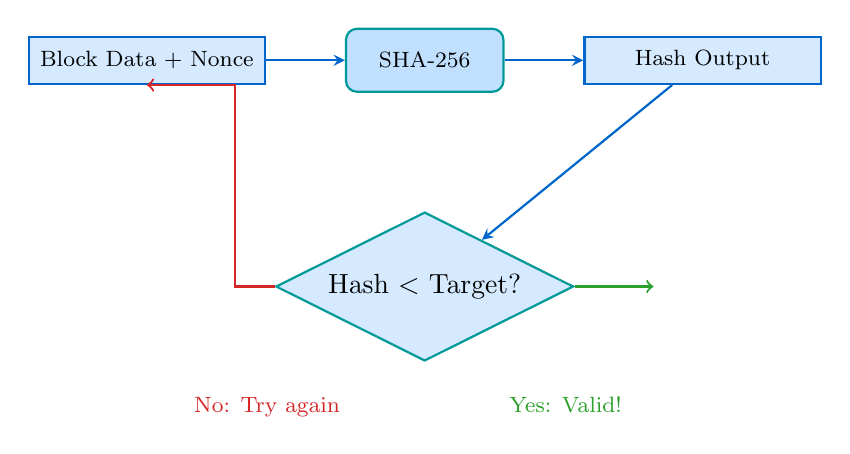
\begin{tikzpicture}[node distance=0.5cm]
% Mining process
\node[databox, minimum width=3cm] (block) {Block Data + Nonce};
\node[hashbox, right=1cm of block, minimum width=2cm] (hash) {SHA-256};
\node[databox, right=1cm of hash, minimum width=3cm] (output) {Hash Output};

\draw[arrow] (block) -- (hash);
\draw[arrow] (hash) -- (output);

% Condition
\node[decision, below=1.5cm of hash, minimum width=2.5cm, aspect=2] (check) {Hash $<$ Target?};

% Outcomes
\node[below left=0.8cm and 0cm of check, font=\footnotesize, text=dfred] (no) {No: Try again};
\node[below right=0.8cm and 0cm of check, font=\footnotesize, text=dfgreen] (yes) {Yes: Valid!};

\draw[arrow] (output) -- (check);
\draw[thick, dfred, ->] (check.west) -- ++(-0.5,0) |- (block.south);
\draw[thick, dfgreen, ->] (check.east) -- ++(1,0);
\end{tikzpicture}
\end{center}

\vspace{3mm}
\textbf{The ``work'' in Proof of Work:}
\begin{itemize}
\item Find a nonce that makes the block hash start with many zeros
\item Requires billions of guesses (brute force)
\item Easy to verify: just hash once and check
\item Hard to produce: requires massive computation
\end{itemize}
\end{frame}

% =======================================================================
% SLIDE 13: MINING EXPLAINED
% =======================================================================
\begin{frame}{Mining: Finding the Golden Nonce}
\textbf{What miners actually do:}

\begin{center}
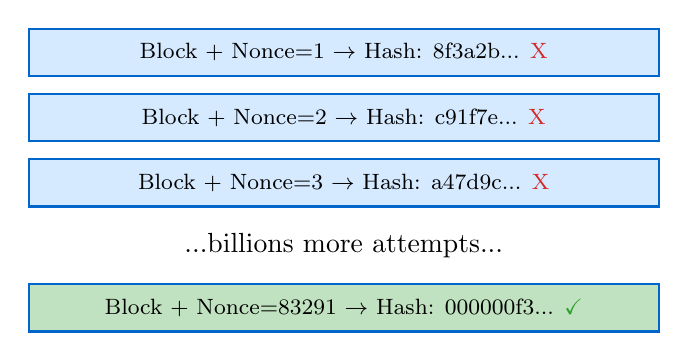
\begin{tikzpicture}[node distance=0.3cm]
% Attempts
\node[databox, minimum width=8cm] (try1) {Block + Nonce=1 $\rightarrow$ Hash: 8f3a2b... \textcolor{dfred}{X}};
\node[databox, minimum width=8cm, below=0.2cm of try1] (try2) {Block + Nonce=2 $\rightarrow$ Hash: c91f7e... \textcolor{dfred}{X}};
\node[databox, minimum width=8cm, below=0.2cm of try2] (try3) {Block + Nonce=3 $\rightarrow$ Hash: a47d9c... \textcolor{dfred}{X}};
\node[below=0.2cm of try3] (dots) {...billions more attempts...};
\node[databox, minimum width=8cm, below=0.2cm of dots, fill=dfgreen!30] (success) {Block + Nonce=83291 $\rightarrow$ Hash: 000000f3... \textcolor{dfgreen}{\checkmark}};
\end{tikzpicture}
\end{center}

\vspace{3mm}
\textbf{Key points:}
\begin{itemize}
\item Nonce = ``Number used once'' -- a value miners keep changing
\item Target = How many leading zeros required (sets difficulty)
\item Finding a valid hash is like winning a lottery
\item Winner gets to add the block and earns rewards
\end{itemize}

\bottomnote{This is why mining requires enormous computational power and electricity}
\end{frame}

% =======================================================================
% SLIDE 14: POW SECURITY MODEL
% =======================================================================
\begin{frame}{Proof of Work: Security Through Energy}
\begin{columns}[T]
\begin{column}{0.48\textwidth}
\textbf{Why It Works}
\begin{itemize}\compactlist
\item Attack requires controlling 51\% of computing power
\item This costs billions in hardware + electricity
\item Rational: mining honestly is more profitable
\item Economic security: attack cost $>$ potential gain
\end{itemize}

\vspace{3mm}
\textbf{Advantages}
\begin{itemize}\compactlist
\item Battle-tested (Bitcoin since 2009)
\item Highly secure
\item Truly decentralized
\end{itemize}
\end{column}
\begin{column}{0.48\textwidth}
\textbf{Criticisms}
\begin{itemize}\compactlist
\item \textcolor{dfred}{Enormous energy consumption}
\item Bitcoin uses more electricity than some countries
\item Environmental concerns
\item Hardware arms race (specialized ASICs)
\end{itemize}

\vspace{3mm}
\begin{center}
\fbox{\parbox{0.85\textwidth}{\centering
Bitcoin Network:\\
$\approx$ 150 TWh/year\\
{\footnotesize (more than Argentina)}
}}
\end{center}
\end{column}
\end{columns}

\bottomnote{PoW trades energy for security -- the ``work'' is the cost of attack}
\end{frame}

% =======================================================================
% SLIDE 15: DIFFICULTY ADJUSTMENT
% =======================================================================
\begin{frame}{Difficulty Adjustment: Self-Regulating Security}
\textbf{How does the network maintain consistent block times?}

\vspace{3mm}
\begin{center}
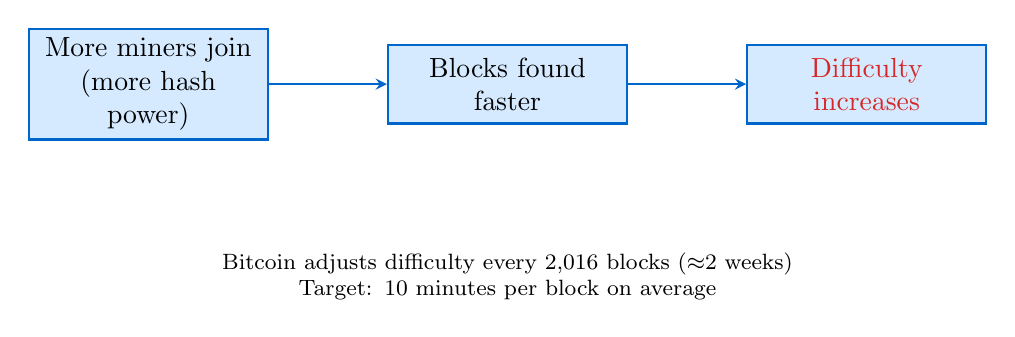
\begin{tikzpicture}[node distance=1cm]
\node[process, minimum width=3cm, text width=2.8cm, align=center] (more) {More miners join\\(more hash power)};
\node[process, minimum width=3cm, text width=2.8cm, align=center, right=1.5cm of more] (fast) {Blocks found\\faster};
\node[process, minimum width=3cm, text width=2.8cm, align=center, right=1.5cm of fast] (inc) {\textcolor{dfred}{Difficulty\\increases}};

\draw[arrow] (more) -- (fast);
\draw[arrow] (fast) -- (inc);

\node[below=1.5cm of fast, font=\footnotesize, text width=8cm, align=center] {
Bitcoin adjusts difficulty every 2,016 blocks ($\approx$2 weeks)\\
Target: 10 minutes per block on average
};
\end{tikzpicture}
\end{center}

\vspace{3mm}
\begin{columns}[T]
\begin{column}{0.48\textwidth}
\textbf{If blocks are too fast:}
\begin{itemize}\compactlist
\item Difficulty increases
\item Requires more leading zeros
\item Harder to find valid hash
\end{itemize}
\end{column}
\begin{column}{0.48\textwidth}
\textbf{If blocks are too slow:}
\begin{itemize}\compactlist
\item Difficulty decreases
\item Requires fewer leading zeros
\item Easier to find valid hash
\end{itemize}
\end{column}
\end{columns}
\end{frame}

% =======================================================================
% SLIDE 16: PROOF OF STAKE - VISUAL
% =======================================================================
\begin{frame}{Proof of Stake (PoS): Ethereum's Answer}
\begin{center}
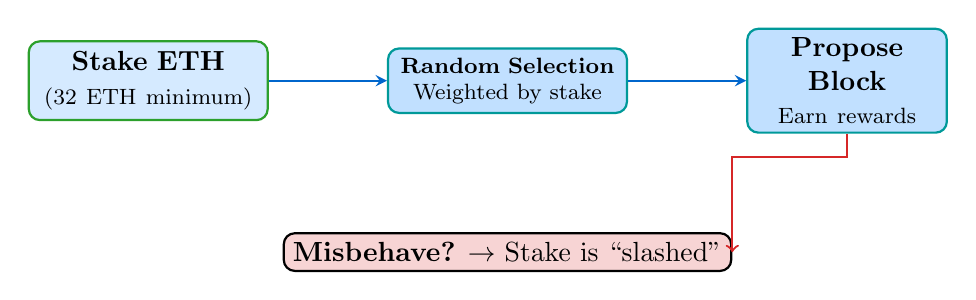
\begin{tikzpicture}[node distance=0.8cm]
% Staking process
\node[walletbox, minimum width=3cm, text width=2.8cm, align=center] (stake) {
\textbf{Stake ETH}\\
\footnotesize (32 ETH minimum)
};

\node[hashbox, right=1.5cm of stake, minimum width=3cm, text width=2.8cm, align=center] (select) {
\textbf{Random Selection}\\
\footnotesize Weighted by stake
};

\node[blocknode, right=1.5cm of select, minimum width=2.5cm, minimum height=1.2cm, text width=2.3cm, align=center] (propose) {
\textbf{Propose Block}\\
\footnotesize Earn rewards
};

\draw[arrow] (stake) -- (select);
\draw[arrow] (select) -- (propose);

% Slashing
\node[below=1.5cm of select, draw, thick, rounded corners, fill=dfred!20, minimum width=5cm] (slash) {
\textbf{Misbehave?} $\rightarrow$ Stake is ``slashed''
};
\draw[thick, dfred, ->] (propose.south) -- ++(0,-0.3) -| (slash.east);
\end{tikzpicture}
\end{center}

\vspace{3mm}
\textbf{The ``stake'' in Proof of Stake:}
\begin{itemize}
\item Lock up cryptocurrency as collateral
\item More stake = higher chance to be selected as validator
\item Honest behavior = earn rewards
\item Malicious behavior = lose your stake (``slashing'')
\end{itemize}
\end{frame}

% =======================================================================
% SLIDE 17: HOW POS WORKS
% =======================================================================
\begin{frame}{How Proof of Stake Works}
\begin{columns}[T]
\begin{column}{0.55\textwidth}
\textbf{Step-by-Step Process:}
\begin{enumerate}
\item \textbf{Stake:} Lock cryptocurrency as collateral
\item \textbf{Selection:} Protocol randomly selects a validator (weighted by stake -- the more coins you lock up, the higher your chance of being selected, like having more lottery tickets)
\item \textbf{Propose:} Selected validator creates a new block
\item \textbf{Attest:} Other validators verify and vote on the block
\item \textbf{Finalize:} Block is added when enough validators agree
\end{enumerate}

\vspace{3mm}
\textbf{Economic Security:}
\begin{itemize}\compactlist
\item Attack requires owning 51\% of staked coins
\item Cheaters lose their stake (slashing)
\item ``Skin in the game'' aligns incentives
\end{itemize}
\end{column}
\begin{column}{0.42\textwidth}
\begin{center}
\fbox{\parbox{0.95\textwidth}{
\textbf{Ethereum PoS Stats:}\\[2mm]
Minimum stake: 32 ETH\\
Total staked: $\sim$30M ETH\\
Active validators: $\sim$900,000\\
Energy reduction: $\sim$99.95\%\\[2mm]
\footnotesize (vs. Proof of Work)
}}
\end{center}

\vspace{3mm}
\textbf{Slashing Penalties:}
\begin{itemize}\compactlist
\item Double signing: Major penalty
\item Being offline: Minor penalty
\item Coordinated attack: Severe penalty
\end{itemize}
\end{column}
\end{columns}
\end{frame}

% =======================================================================
% SLIDE 18: POW VS POS COMPARISON
% =======================================================================
\begin{frame}{PoW vs. PoS: Head-to-Head Comparison}
\begin{center}
\begin{tabular}{l|c|c}
\toprule
\textbf{Aspect} & \textbf{Proof of Work} & \textbf{Proof of Stake} \\
\midrule
Security basis & Computational power & Economic stake \\
Energy usage & \textcolor{dfred}{Very high} & \textcolor{dfgreen}{Low ($\sim$99.9\% less)} \\
Hardware required & Specialized (ASICs) & Standard computers \\
Entry barrier & High (equipment cost) & High (32 ETH $\approx$ \$60k) \\
Attack cost & Hardware + electricity & Acquire 51\% of stake \\
Decentralization & Mining pool concentration & Wealth concentration \\
Finality & Probabilistic & Faster, more definite \\
Examples & Bitcoin, Dogecoin & Ethereum, Cardano, Solana \\
\bottomrule
\end{tabular}
\end{center}

\vspace{3mm}
\textbf{Key insight:} Neither is ``better'' -- they make different tradeoffs

\bottomnote{Ethereum transitioned from PoW to PoS in Sept 2022 (``The Merge'')}
\end{frame}

% =======================================================================
% SLIDE 19: THE LONGEST CHAIN RULE
% =======================================================================
\begin{frame}{The Longest Chain Rule}
\textbf{How does the network resolve conflicts?}

\vspace{3mm}
\begin{center}
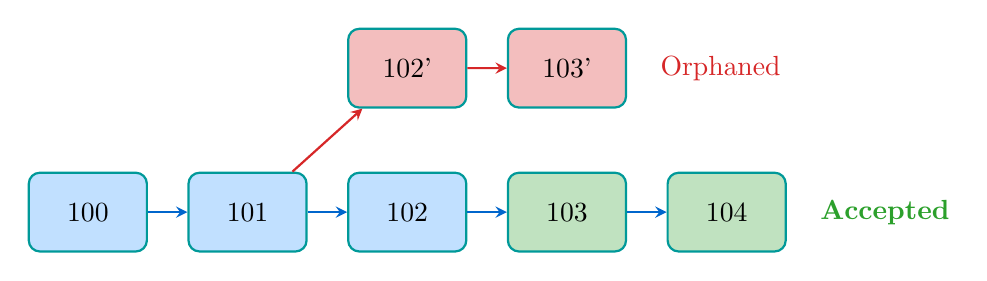
\begin{tikzpicture}[scale=0.8, node distance=0.3cm]
% Main chain
\node[blocknode, minimum width=1.5cm, minimum height=1cm] (b1) {100};
\node[blocknode, minimum width=1.5cm, minimum height=1cm, right=0.5cm of b1] (b2) {101};
\node[blocknode, minimum width=1.5cm, minimum height=1cm, right=0.5cm of b2] (b3) {102};
\node[blocknode, minimum width=1.5cm, minimum height=1cm, right=0.5cm of b3, fill=dfgreen!30] (b4) {103};
\node[blocknode, minimum width=1.5cm, minimum height=1cm, right=0.5cm of b4, fill=dfgreen!30] (b5) {104};

% Fork
\node[blocknode, minimum width=1.5cm, minimum height=1cm, above right=0.8cm and 0.5cm of b2, fill=dfred!30] (f1) {102'};
\node[blocknode, minimum width=1.5cm, minimum height=1cm, right=0.5cm of f1, fill=dfred!30] (f2) {103'};

\draw[arrow] (b1) -- (b2);
\draw[arrow] (b2) -- (b3);
\draw[arrow] (b3) -- (b4);
\draw[arrow] (b4) -- (b5);
\draw[arrow, dfred] (b2) -- (f1);
\draw[arrow, dfred] (f1) -- (f2);

% Labels
\node[right=0.3cm of b5, text=dfgreen] {\textbf{Accepted}};
\node[right=0.3cm of f2, text=dfred] {Orphaned};
\end{tikzpicture}
\end{center}

\vspace{3mm}
\begin{columns}[T]
\begin{column}{0.55\textwidth}
\textbf{The Rule:}
\begin{itemize}\compactlist
\item Nodes accept the chain with \textbf{most cumulative work}
\item In PoW: typically the longest chain
\item In PoS: chain with most validator votes
\item Shorter chains become ``orphaned''
\end{itemize}
\end{column}
\begin{column}{0.42\textwidth}
\textbf{Why It Works:}
\begin{itemize}\compactlist
\item Provides decentralized consensus
\item Resolves temporary forks
\item Makes 51\% attacks expensive
\item No voting or coordination needed
\end{itemize}
\end{column}
\end{columns}
\end{frame}

% =======================================================================
% SLIDE 20: CONFIRMATION DEPTH
% =======================================================================
\begin{frame}{Confirmation Depth: How Secure Is Your Transaction?}
\textbf{More confirmations = More security}

\vspace{3mm}
\begin{center}
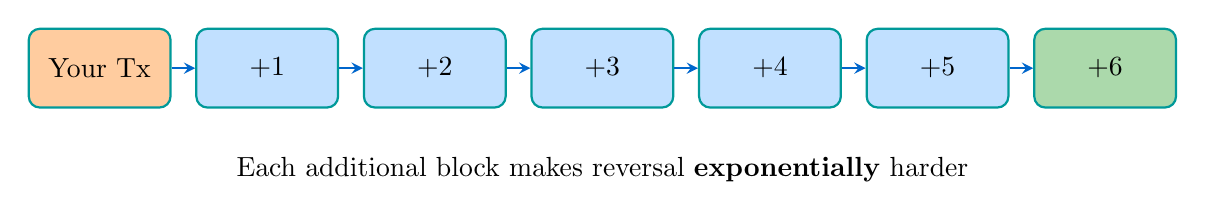
\begin{tikzpicture}[scale=0.75, node distance=0.2cm]
\node[blocknode, minimum width=1.8cm, minimum height=1cm, fill=dforange!40] (tx) {Your Tx};
\node[blocknode, minimum width=1.8cm, minimum height=1cm, right=0.3cm of tx] (c1) {+1};
\node[blocknode, minimum width=1.8cm, minimum height=1cm, right=0.3cm of c1] (c2) {+2};
\node[blocknode, minimum width=1.8cm, minimum height=1cm, right=0.3cm of c2] (c3) {+3};
\node[blocknode, minimum width=1.8cm, minimum height=1cm, right=0.3cm of c3] (c4) {+4};
\node[blocknode, minimum width=1.8cm, minimum height=1cm, right=0.3cm of c4] (c5) {+5};
\node[blocknode, minimum width=1.8cm, minimum height=1cm, right=0.3cm of c5, fill=dfgreen!40] (c6) {+6};

\draw[arrow] (tx) -- (c1);
\draw[arrow] (c1) -- (c2);
\draw[arrow] (c2) -- (c3);
\draw[arrow] (c3) -- (c4);
\draw[arrow] (c4) -- (c5);
\draw[arrow] (c5) -- (c6);

\node[below=0.5cm of c3, text width=10cm, align=center] {
Each additional block makes reversal \textbf{exponentially} harder
};
\end{tikzpicture}
\end{center}

\vspace{3mm}
\begin{center}
\begin{tabular}{l|c|l}
\toprule
\textbf{Confirmations} & \textbf{Time (BTC)} & \textbf{Typical Use} \\
\midrule
0 (unconfirmed) & 0 min & Very small amounts only \\
1 confirmation & 10 min & Low-value transactions \\
3 confirmations & 30 min & Medium-value transactions \\
\textbf{6 confirmations} & 60 min & \textbf{Industry standard for security} \\
\bottomrule
\end{tabular}
\end{center}
\end{frame}

% =======================================================================
% SLIDE 21: 51% ATTACK
% =======================================================================
\begin{frame}{The 51\% Attack: Understanding the Risk}
\textbf{What is a 51\% attack?}

An attacker controlling $>$50\% of network hash power (PoW) or stake (PoS) can:

\vspace{3mm}
\begin{columns}[T]
\begin{column}{0.48\textwidth}
\textbf{What they CAN do:}
\begin{itemize}\compactlist
\item \textcolor{dfred}{Double-spend} their own coins
\item \textcolor{dfred}{Block} other transactions (censorship)
\item \textcolor{dfred}{Reorganize} recent blocks
\item Prevent confirmations
\end{itemize}
\end{column}
\begin{column}{0.48\textwidth}
\textbf{What they CANNOT do:}
\begin{itemize}\compactlist
\item \textcolor{dfgreen}{Steal} other people's coins
\item \textcolor{dfgreen}{Create} coins out of nothing
\item \textcolor{dfgreen}{Change} consensus rules
\item Reverse very old transactions
\end{itemize}
\end{column}
\end{columns}

\vspace{5mm}
\begin{block}{Economic Reality}
For Bitcoin, acquiring 51\% hash power would cost billions of dollars in hardware and ongoing electricity. The attack would likely destroy the value of the attacker's own coins -- making it economically irrational.
\end{block}
\end{frame}

% =======================================================================
% SLIDE 22: THE BLOCKCHAIN TRILEMMA
% =======================================================================
\begin{frame}{The Blockchain Trilemma}
\begin{center}
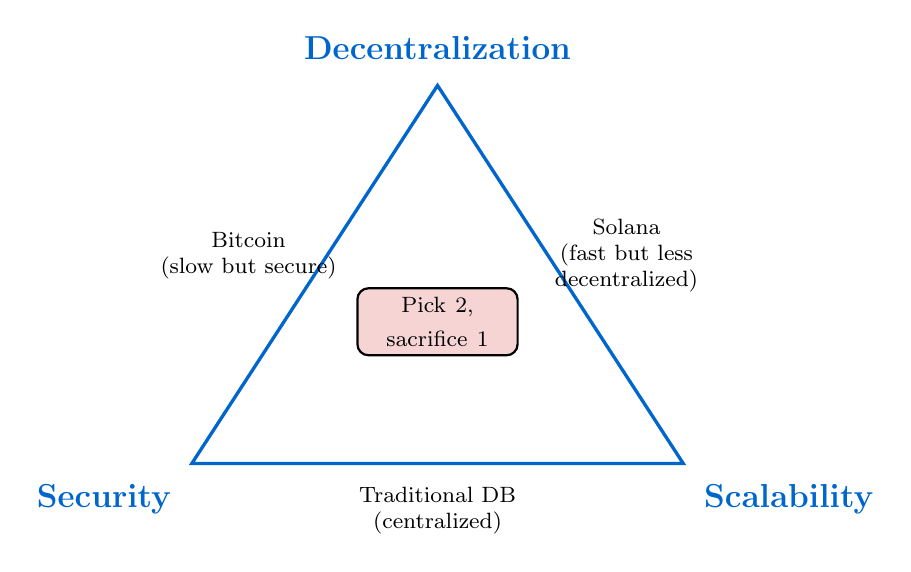
\begin{tikzpicture}[scale=1.2]
% Triangle
\coordinate (D) at (0, 3);
\coordinate (Se) at (-2.6, -1);
\coordinate (Sc) at (2.6, -1);

\draw[very thick, dfblue] (D) -- (Se) -- (Sc) -- cycle;

% Labels
\node[above=2mm of D, font=\bfseries\large, text=dfblue] {Decentralization};
\node[below left=2mm of Se, font=\bfseries\large, text=dfblue] {Security};
\node[below right=2mm of Sc, font=\bfseries\large, text=dfblue] {Scalability};

% Center impossible zone
\node[draw, thick, rounded corners, fill=dfred!20, minimum width=2cm, text width=1.8cm, align=center] at (0, 0.5) {
\footnotesize Pick 2,\\
sacrifice 1
};

% Examples on edges
\node[font=\footnotesize, text width=2.3cm, align=center] at (-2, 1.2) {Bitcoin\\(slow but secure)};
\node[font=\footnotesize, text width=2.3cm, align=center] at (2, 1.2) {Solana\\(fast but less\\decentralized)};
\node[font=\footnotesize, text width=2.3cm, align=center] at (0, -1.5) {Traditional DB\\(centralized)};
\end{tikzpicture}
\end{center}
\end{frame}

% =======================================================================
% SLIDE 23: TRILEMMA EXPLAINED
% =======================================================================
\begin{frame}{The Trilemma Explained}
\begin{columns}[T]
\begin{column}{0.32\textwidth}
\textbf{Decentralization}
\begin{itemize}\compactlist
\item Many independent validators
\item No single point of control
\item Censorship resistant
\item Geographic distribution
\end{itemize}
\textcolor{dfred}{Tradeoff: More nodes = slower}
\end{column}
\begin{column}{0.32\textwidth}
\textbf{Security}
\begin{itemize}\compactlist
\item Resistant to attacks
\item Immutable history
\item Byzantine fault tolerant
\item Economic finality
\end{itemize}
\textcolor{dfred}{Tradeoff: More verification = slower}
\end{column}
\begin{column}{0.32\textwidth}
\textbf{Scalability}
\begin{itemize}\compactlist
\item High throughput (Transactions Per Second -- TPS)
\item Low latency
\item Low fees
\item Handle demand spikes
\end{itemize}
\textcolor{dfred}{Tradeoff: Speed often requires centralization}
\end{column}
\end{columns}

\vspace{5mm}
\textbf{Performance comparison:} Compare how different systems balance speed, certainty, and decentralization

\vspace{2mm}
\begin{center}
\begin{tabular}{l|ccc}
\toprule
\textbf{System} & \textbf{TPS} & \textbf{Finality*} & \textbf{Validators} \\
\midrule
Bitcoin & 7 & 60 min & $\sim$15,000 nodes \\
Ethereum & 15-30 & 12-15 min & $\sim$500,000 validators \\
Solana & 65,000 & 0.4 sec & $\sim$1,900 validators \\
Visa & 24,000 & seconds & 1 (centralized) \\
\bottomrule
\end{tabular}

\vspace{2mm}
\footnotesize *Finality = when a transaction becomes permanent and irreversible
\end{center}
\end{frame}

% =======================================================================
% SLIDE 24: SCALING SOLUTIONS
% =======================================================================
\begin{frame}{Scaling Solutions: Breaking the Trilemma?}
\textit{These solutions are still evolving -- the key idea is that blockchains face a speed/security/decentralization tradeoff.}

\vspace{2mm}
\begin{columns}[T]
\begin{column}{0.48\textwidth}
\textbf{Layer 1 Solutions}

\textit{Improve the base blockchain}
\begin{itemize}\compactlist
\item Larger blocks (more data per block)
\item Faster block times
\item More efficient consensus
\item Sharding* (parallel processing)
\end{itemize}

\vspace{3mm}
\textbf{Examples:}
\begin{itemize}\compactlist
\item Ethereum 2.0 (sharding planned)
\item Solana (parallel processing)
\item Near Protocol (sharding)
\end{itemize}
\end{column}
\begin{column}{0.48\textwidth}
\textbf{Layer 2 Solutions}

\textit{Build on top of base layer}
\begin{itemize}\compactlist
\item Process transactions off-chain
\item Settle on main chain periodically
\item Inherit security from L1
\item Much higher throughput
\end{itemize}

\vspace{3mm}
\textbf{Examples:}
\begin{itemize}\compactlist
\item Lightning Network (Bitcoin)
\item Optimism, Arbitrum (rollups*)
\item Polygon (sidechain*)
\end{itemize}
\end{column}
\end{columns}

\vspace{1mm}
{\scriptsize *Sharding = splitting the network into parallel sections. Rollups = bundling many transactions into one. Sidechains = separate chains connected to the main one.}

\vspace{1mm}
\begin{block}{Key Insight}
Layer 2 solutions let blockchains scale WITHOUT sacrificing decentralization or security at the base layer.
\end{block}
\end{frame}

% =======================================================================
% SLIDE 25: HANDS-ON EXERCISE - NB06 INTRO
% =======================================================================
\begin{frame}{Hands-On Exercise: Blockchain Simulation (NB06)}
\textbf{In this notebook, you will:}

\begin{enumerate}
\item \textbf{Build a block} -- Create a simple block data structure with all required fields
\vspace{2mm}
\item \textbf{Create a chain} -- Link multiple blocks together using hash pointers
\vspace{2mm}
\item \textbf{Attempt tampering} -- Modify a block and observe chain validation failure
\vspace{2mm}
\item \textbf{Simulate mining} -- Implement a simple Proof of Work algorithm
\vspace{2mm}
\item \textbf{Adjust difficulty} -- See how difficulty affects mining time
\end{enumerate}

\vspace{5mm}
\begin{center}
\fbox{\parbox{0.8\textwidth}{\centering
\textbf{Learning Goal:} Understand blockchain mechanics through hands-on coding, not just theory.
}}
\end{center}

\bottomnote{Open NB06\_blockchain\_simulation.ipynb in Google Colab}
\end{frame}

% =======================================================================
% SLIDE 26: HANDS-ON EXERCISE - WHAT TO EXPECT
% =======================================================================
\begin{frame}{NB06: What You'll Build}
\begin{columns}[T]
\begin{column}{0.55\textwidth}
\textbf{Block Class Structure:}
\begin{itemize}\compactlist
\item Index, timestamp, data
\item Previous hash, nonce
\item Calculated hash
\end{itemize}

\vspace{3mm}
\textbf{Blockchain Class:}
\begin{itemize}\compactlist
\item Genesis block creation
\item Adding new blocks
\item Chain validation
\item Tampering detection
\end{itemize}

\vspace{3mm}
\textbf{Mining Simulation:}
\begin{itemize}\compactlist
\item Find valid nonce
\item Meet difficulty target
\item Measure iterations
\end{itemize}
\end{column}
\begin{column}{0.42\textwidth}
\begin{center}
\fbox{\parbox{0.95\textwidth}{
\textbf{Expected Observations:}\\[2mm]
\footnotesize
1. Changing one character breaks the entire chain\\[1mm]
2. Mining difficulty dramatically affects time\\[1mm]
3. Verification is instant; creation is hard\\[1mm]
4. Longer chains resist tampering better
}}
\end{center}

\vspace{3mm}
\textbf{Time estimate:} 30-45 minutes

\textbf{Prerequisites:} Basic Python, completed T3.1
\end{column}
\end{columns}
\end{frame}

% =======================================================================
% SLIDE 27: DISCUSSION - REAL WORLD APPLICATIONS
% =======================================================================
\begin{frame}{Discussion: Blockchain in the Real World}
\textbf{Where does blockchain make sense?}

\vspace{3mm}
\begin{columns}[T]
\begin{column}{0.48\textwidth}
\textbf{Good Use Cases:}
\begin{itemize}\compactlist
\item \textcolor{dfgreen}{Permissionless value transfer}
\item \textcolor{dfgreen}{Trustless coordination}
\item \textcolor{dfgreen}{Censorship-resistant applications}
\item \textcolor{dfgreen}{Transparent audit trails}
\item \textcolor{dfgreen}{Programmable money (smart contracts)}
\end{itemize}
\end{column}
\begin{column}{0.48\textwidth}
\textbf{Poor Use Cases:}
\begin{itemize}\compactlist
\item \textcolor{dfred}{High-speed trading}
\item \textcolor{dfred}{Private data storage}
\item \textcolor{dfred}{When trust already exists}
\item \textcolor{dfred}{When centralization is acceptable}
\item \textcolor{dfred}{When efficiency matters most}
\end{itemize}
\end{column}
\end{columns}

\vspace{5mm}
\begin{block}{Key Question}
Before choosing blockchain, ask: ``Is the inefficiency worth the trust minimization?''
\end{block}
\end{frame}

% =======================================================================
% SLIDE 28: DISCUSSION - ENVIRONMENTAL DEBATE
% =======================================================================
\begin{frame}{Discussion: The Energy Debate}
\textbf{Is Proof of Work's energy use justified?}

\vspace{3mm}
\begin{columns}[T]
\begin{column}{0.48\textwidth}
\textbf{Arguments FOR PoW:}
\begin{itemize}\compactlist
\item Energy = security; necessary cost
\item Bitcoin increasingly uses renewables
\item Traditional finance also uses energy
\item Monetary sovereignty has value
\item Market decides if cost is worth it
\end{itemize}
\end{column}
\begin{column}{0.48\textwidth}
\textbf{Arguments AGAINST PoW:}
\begin{itemize}\compactlist
\item Environmental impact is real
\item PoS achieves similar security
\item E-waste from mining hardware
\item Energy could be used elsewhere
\item Alternatives exist and work
\end{itemize}
\end{column}
\end{columns}

\vspace{5mm}
\begin{center}
\fbox{\parbox{0.85\textwidth}{\centering
\textbf{The Merge (Sept 2022):} Ethereum's switch from PoW to PoS reduced its energy consumption by $\sim$99.95\%, proving that high security doesn't require high energy.
}}
\end{center}
\end{frame}

% =======================================================================
% SLIDE 29: DISCUSSION - DECENTRALIZATION SPECTRUM
% =======================================================================
\begin{frame}{Discussion: How Decentralized Is ``Decentralized''?}
\textbf{Decentralization is a spectrum, not binary:}

\begin{center}
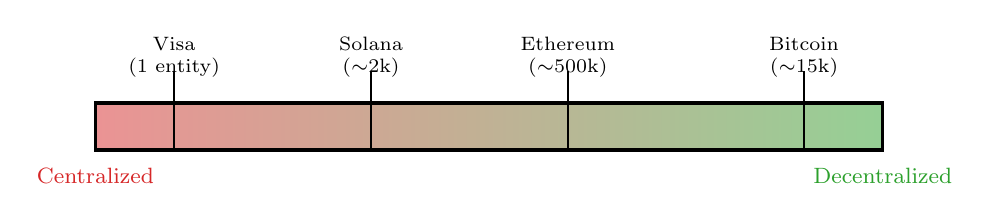
\begin{tikzpicture}
% Spectrum bar
\draw[very thick, left color=dfred!50, right color=dfgreen!50] (-5,-0.3) rectangle (5,0.3);
\node[below=0.4cm, font=\footnotesize, text=dfred] at (-5,0) {Centralized};
\node[below=0.4cm, font=\footnotesize, text=dfgreen] at (5,0) {Decentralized};

% Markers
\node[above=0.5cm, font=\scriptsize, text width=1.5cm, align=center] at (-4, 0) {Visa\\(1 entity)};
\node[above=0.5cm, font=\scriptsize, text width=1.5cm, align=center] at (-1.5, 0) {Solana\\($\sim$2k)};
\node[above=0.5cm, font=\scriptsize, text width=1.8cm, align=center] at (1, 0) {Ethereum\\($\sim$500k)};
\node[above=0.5cm, font=\scriptsize, text width=1.5cm, align=center] at (4, 0) {Bitcoin\\($\sim$15k)};

\draw[thick] (-4, -0.3) -- (-4, 0.7);
\draw[thick] (-1.5, -0.3) -- (-1.5, 0.7);
\draw[thick] (1, -0.3) -- (1, 0.7);
\draw[thick] (4, -0.3) -- (4, 0.7);
\end{tikzpicture}
\end{center}

\vspace{5mm}
\textbf{Questions to consider:}
\begin{itemize}
\item How many entities control $>$50\% of validation power?
\item Can one entity censor transactions?
\item What's the geographic distribution of nodes?
\item Who controls the protocol development?
\end{itemize}
\end{frame}

% =======================================================================
% SLIDE 30: DISCUSSION - FUTURE OF CONSENSUS
% =======================================================================
\begin{frame}{Discussion: The Future of Consensus Mechanisms}
\textbf{What's next for blockchain consensus?}

\vspace{3mm}
\begin{columns}[T]
\begin{column}{0.48\textwidth}
\textbf{Current Research Areas:}
\begin{itemize}\compactlist
\item \textbf{Hybrid consensus:} Combine PoW and PoS
\item \textbf{DAG-based*:} IOTA, Hedera
\item \textbf{BFT variants:} Faster finality
\item \textbf{Privacy + scale:} Covered in Day 4
\end{itemize}

\vspace{3mm}
\textbf{Emerging Solutions:}
\begin{itemize}\compactlist
\item Rollups (bundling transactions)
\item Data availability sampling**
\item Cross-chain bridges
\end{itemize}

{\scriptsize *DAG = Directed Acyclic Graph -- a different data structure where multiple blocks can be added in parallel.\\
**Checking that data exists without downloading all of it.}
\end{column}
\begin{column}{0.48\textwidth}
\textbf{Open Questions:}
\begin{itemize}
\item Can we truly solve the trilemma?
\item How will regulation affect consensus choice?
\item Will institutional adoption favor certain mechanisms?
\item Can decentralization survive mainstream adoption?
\end{itemize}

\vspace{3mm}
\textcolor{dfblue}{\textit{The consensus mechanism debate will shape the future of digital finance.}}
\end{column}
\end{columns}
\end{frame}

% =======================================================================
% SLIDE 31: EXECUTIVE SUMMARY
% =======================================================================
\begin{frame}{Executive Summary: Key Takeaways}
\begin{enumerate}
\item \textbf{Blockchain = Distributed + Append-only + Consensus}\\
A chain of cryptographically linked blocks maintained by thousands of nodes without central authority.

\vspace{3mm}
\item \textbf{Immutability comes from hash linking}\\
Changing any block invalidates all subsequent blocks, making tampering detectable and economically prohibitive.

\vspace{3mm}
\item \textbf{Consensus mechanisms solve the trust problem}\\
PoW uses computational work; PoS uses economic stake. Both create costs for attackers.

\vspace{3mm}
\item \textbf{The trilemma forces design tradeoffs}\\
No blockchain can maximize decentralization, security, AND scalability simultaneously.

\vspace{3mm}
\item \textbf{Layer 2 solutions offer scalability without compromise}\\
Build fast systems on top of secure base layers.
\end{enumerate}
\end{frame}

% =======================================================================
% SLIDE 32: CONCEPT MAP
% =======================================================================
\begin{frame}{Concept Map: Blockchain Components}
\begin{center}
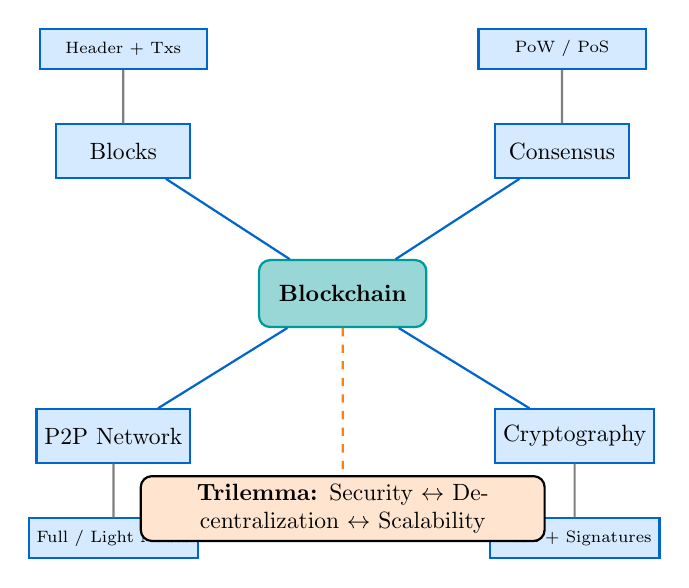
\begin{tikzpicture}[scale=0.85, transform shape, node distance=1.2cm]
% Central node
\node[blocknode, minimum width=2.5cm, minimum height=1cm, fill=dfteal!40] (bc) {\textbf{Blockchain}};

% Layer 1 nodes
\node[process, minimum width=2cm, minimum height=0.8cm, above left=1.2cm and 1cm of bc] (blocks) {Blocks};
\node[process, minimum width=2cm, minimum height=0.8cm, above right=1.2cm and 1cm of bc] (consensus) {Consensus};
\node[process, minimum width=2cm, minimum height=0.8cm, below left=1.2cm and 1cm of bc] (network) {P2P Network};
\node[process, minimum width=2cm, minimum height=0.8cm, below right=1.2cm and 1cm of bc] (crypto) {Cryptography};

% Layer 2 nodes
\node[databox, above=0.8cm of blocks, font=\scriptsize] (header) {Header + Txs};
\node[databox, above=0.8cm of consensus, font=\scriptsize] (pow) {PoW / PoS};
\node[databox, below=0.8cm of network, font=\scriptsize] (nodes) {Full / Light Nodes};
\node[databox, below=0.8cm of crypto, font=\scriptsize] (hash) {Hash + Signatures};

% Connections to center
\draw[thick, dfblue] (bc) -- (blocks);
\draw[thick, dfblue] (bc) -- (consensus);
\draw[thick, dfblue] (bc) -- (network);
\draw[thick, dfblue] (bc) -- (crypto);

% Connections to outer
\draw[thick, dfgray] (blocks) -- (header);
\draw[thick, dfgray] (consensus) -- (pow);
\draw[thick, dfgray] (network) -- (nodes);
\draw[thick, dfgray] (crypto) -- (hash);

% Trilemma at bottom
\node[below=2.2cm of bc, draw, thick, rounded corners, fill=dforange!20, minimum width=6cm, text width=5.8cm, align=center] (trilemma) {
\textbf{Trilemma:} Security $\leftrightarrow$ Decentralization $\leftrightarrow$ Scalability
};
\draw[thick, dforange, dashed] (bc) -- (trilemma);
\end{tikzpicture}
\end{center}
\end{frame}

% =======================================================================
% SLIDE 33: KEY TERMS 1
% =======================================================================
\begin{frame}{Key Terms \& Definitions (1/2)}
\begin{description}
\item[Blockchain] A distributed ledger of cryptographically linked blocks maintained by consensus among network participants.

\item[Block] A data structure containing transactions, a timestamp, and a reference to the previous block via its hash.

\item[Genesis Block] The first block in a blockchain (Block 0), which has no previous block to reference.

\item[Consensus Mechanism] A protocol enabling distributed nodes to agree on the state of the ledger without central authority.

\item[Proof of Work (PoW)] Consensus mechanism requiring computational effort to find a hash meeting difficulty requirements.
\end{description}
\end{frame}

% =======================================================================
% SLIDE 34: KEY TERMS 2
% =======================================================================
\begin{frame}{Key Terms \& Definitions (2/2)}
\begin{description}
\item[Proof of Stake (PoS)] Consensus mechanism where validators stake cryptocurrency as collateral; misbehavior results in ``slashing.''

\item[Nonce] ``Number used once'' -- a value miners vary to find a valid block hash in Proof of Work.

\item[51\% Attack] When an attacker controls majority hash power/stake, enabling double-spending or censorship.

\item[Blockchain Trilemma] The observation that blockchains can optimize at most two of: decentralization, security, scalability.

\item[Layer 2] Protocols built on top of a base blockchain to increase throughput while inheriting L1 security.
\end{description}
\end{frame}

% =======================================================================
% SLIDE 35: COMMON MISCONCEPTIONS
% =======================================================================
\begin{frame}{Common Misconceptions}
\begin{tabular}{p{5cm}|p{5.5cm}}
\textbf{Myth} & \textbf{Reality} \\
\hline
& \\
``Blockchain data is encrypted'' & Blockchain data is \textbf{public and transparent}. Anyone can read all transactions. Privacy requires additional layers. \\[3mm]
\hline
& \\
``51\% attackers can steal coins'' & Attackers can only \textbf{double-spend their own coins} or censor transactions. They cannot steal from others. \\[3mm]
\hline
& \\
``PoS is always better than PoW'' & Each makes \textbf{different tradeoffs}. PoS is more efficient but has different centralization risks. \\[3mm]
\hline
& \\
``Blockchain is infinitely scalable'' & The \textbf{trilemma is real}. Scaling requires tradeoffs or Layer 2 solutions. \\
\end{tabular}
\end{frame}

% =======================================================================
% SLIDE 36: SELF-ASSESSMENT 1
% =======================================================================
\begin{frame}{Self-Assessment Questions (1/2)}
\textbf{Question 1:} Which of the following are components of a block's structure?

\vspace{2mm}
\begin{enumerate}[A.]
\item Only the transaction data and timestamp
\item Index, timestamp, data, previous hash, nonce, and current hash
\item Only the cryptographic hash and signature
\item Public key, private key, and transaction list
\end{enumerate}

\vspace{5mm}
\pause
\textcolor{dfgreen}{\textbf{Answer: B}}

\textit{Explanation:} A block contains multiple components: index (position in chain), timestamp (when created), data (transactions/content), previous hash (link to previous block), nonce (proof-of-work number), and hash (the block's digital fingerprint). All these components work together to create a secure, tamper-evident structure.
\end{frame}

% =======================================================================
% SLIDE 37: SELF-ASSESSMENT 2
% =======================================================================
\begin{frame}{Self-Assessment Questions (2/2)}
\textbf{Question 2:} Describe the hash puzzle solving process in PoW mining.

\vspace{2mm}
\begin{enumerate}[A.]
\item Miners solve complex mathematical equations involving prime numbers
\item Miners repeatedly change the nonce and calculate the block hash until finding one that starts with the required number of zeros
\item Miners decrypt encrypted puzzles using private keys
\item Miners compete to find the shortest hash value
\end{enumerate}

\vspace{3mm}
\pause
\textcolor{dfgreen}{\textbf{Answer: B}}

\textit{Explanation:} The hash puzzle is computationally intensive but simple: find a nonce that produces a hash meeting the difficulty target. Since hash functions are one-way, the only approach is brute force -- incrementing the nonce until finding a valid hash.

\vspace{3mm}
\textbf{Question 3:} What is the genesis block?

\pause
\textcolor{dfgreen}{\textbf{Answer:}} The first block in a blockchain (Block 0), with no previous block to reference.
\end{frame}

% =======================================================================
% SLIDE 38: WHAT'S NEXT
% =======================================================================
\begin{frame}{What's Next: Topic 3.3 -- Wallets \& Transactions}
\textbf{From theory to practice: How users actually interact with blockchains}

\vspace{5mm}
\begin{columns}[T]
\begin{column}{0.48\textwidth}
\textbf{Topics we'll cover:}
\begin{itemize}
\item What is a wallet, really?
\item Hot vs. cold wallets
\item Custodial vs. non-custodial
\item Transaction lifecycle
\item The UX gap problem
\end{itemize}
\end{column}
\begin{column}{0.48\textwidth}
\textbf{Key insight preview:}
\begin{center}
\fbox{\parbox{0.9\textwidth}{
\textbf{Common Misconception:}\\[2mm]
Wallets don't ``store'' cryptocurrency.\\[1mm]
The blockchain stores balances.\\[1mm]
Wallets store \textit{keys} that prove you can spend those balances.
}}
\end{center}
\end{column}
\end{columns}

\vspace{5mm}
\textbf{Connection to today:} Now that you understand how blockchains work internally, we'll explore how users sign and broadcast transactions to interact with them.
\end{frame}

% =======================================================================
% SLIDE 39: RESOURCES
% =======================================================================
\begin{frame}{Resources for Further Learning}
\textbf{Essential Reading:}
\begin{itemize}
\item Nakamoto, S. (2008). \textit{Bitcoin: A Peer-to-Peer Electronic Cash System}
\item Buterin, V. (2014). \textit{Ethereum Whitepaper}
\item Antonopoulos, A. \textit{Mastering Bitcoin} (Chapters 6-10)
\end{itemize}

\vspace{3mm}
\textbf{Interactive Tools:}
\begin{itemize}
\item \textbf{Blockchain Demo:} \url{https://andersbrownworth.com/blockchain/}
\item \textbf{Bitcoin Block Explorer:} \url{https://blockstream.info/}
\item \textbf{Ethereum Block Explorer:} \url{https://etherscan.io/}
\end{itemize}

\vspace{3mm}
\textbf{Videos:}
\begin{itemize}
\item 3Blue1Brown: ``But how does bitcoin actually work?''
\item MIT OpenCourseWare: Blockchain and Money (Gary Gensler)
\end{itemize}

\bottomnote{NB06 provides hands-on practice with the concepts from this lecture}
\end{frame}

% =======================================================================
% SLIDE 40: QUESTIONS
% =======================================================================
\begin{frame}[plain]
\vfill
\begin{center}
{\Huge \textbf{Questions?}}

\vspace{10mm}
{\large Topic 3.2: Blockchain Mechanics}

\vspace{5mm}
{\normalsize Consensus, Blocks, and the Trilemma}

\vspace{10mm}
\textcolor{dfblue}{\textbf{Next:} Topic 3.3 -- Wallets \& Transactions}
\end{center}
\vfill
\end{frame}

\end{document}
